
\tikzset{every picture/.style={line width=0.75pt}} %set default line width to 0.75pt        
\marginnote{
	\begin{minipage}{5.5cm}
		\begin{figure}[H]\centering
	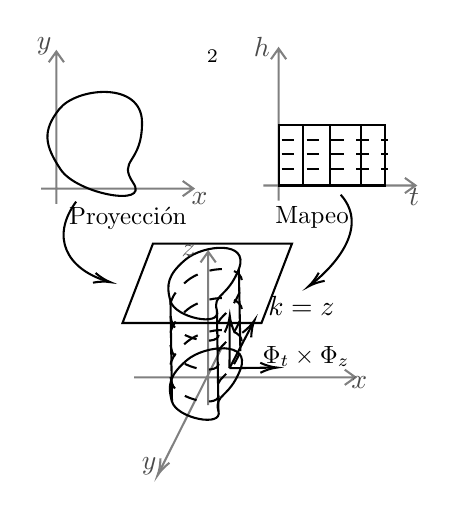
\begin{tikzpicture}[x=0.55pt,y=0.55pt,yscale=-1,xscale=1]
	%uncomment if require: \path (0,300); %set diagram left start at 0, and has height of 300
	
	%Shape: Axis 2D [id:dp0671023438890539] 
	\draw [color={rgb, 255:red, 128; green, 128; blue, 128 }  ,draw opacity=1 ] (23,103.33) -- (123,103.33)(33,13.33) -- (33,113.33) (116,98.33) -- (123,103.33) -- (116,108.33) (28,20.33) -- (33,13.33) -- (38,20.33)  ;
	%Shape: Axis 2D [id:dp4356880068192882] 
	\draw [color={rgb, 255:red, 128; green, 128; blue, 128 }  ,draw opacity=1 ] (169,101.33) -- (269,101.33)(179,11.33) -- (179,111.33) (262,96.33) -- (269,101.33) -- (262,106.33) (174,18.33) -- (179,11.33) -- (184,18.33)  ;
	%Shape: Regular Polygon [id:dp83345563817431] 
	\draw   (34.93,51.11) .. controls (46.22,36.85) and (89.29,32.45) .. (89.29,60.03) .. controls (89.29,87.61) and (72.97,83.82) .. (83.61,99.78) .. controls (94.25,115.74) and (46.45,106.75) .. (35.81,90.79) .. controls (25.18,74.83) and (23.65,65.36) .. (34.93,51.11) -- cycle ;
	%Shape: Rectangle [id:dp9058281148634225] 
	\draw   (179,61.33) -- (249,61.33) -- (249,101.33) -- (179,101.33) -- cycle ;
	%Shape: Boxed Line [id:dp7517627309771912] 
	\draw  [dash pattern={on 4.5pt off 4.5pt}]  (181,90.33) -- (251,90.33) ;
	
	
	%Shape: Boxed Line [id:dp23509819907190233] 
	\draw  [dash pattern={on 4.5pt off 4.5pt}]  (181,80.33) -- (251,80.33) ;
	
	
	%Shape: Boxed Line [id:dp965403871016088] 
	\draw  [dash pattern={on 4.5pt off 4.5pt}]  (181,71.33) -- (251,71.33) ;
	
	
	%Shape: Boxed Bezier Curve [id:dp36220731772572023] 
	\draw    (46.01,111.91) .. controls (28.88,135.18) and (39.6,156.29) .. (66.78,164.36) ;
	\draw [shift={(68.46,164.83)}, rotate = 195.12] [color={rgb, 255:red, 0; green, 0; blue, 0 }  ][line width=0.75]    (10.93,-3.29) .. controls (6.95,-1.4) and (3.31,-0.3) .. (0,0) .. controls (3.31,0.3) and (6.95,1.4) .. (10.93,3.29)   ;
	
	%Curve Lines [id:da22018553388559514] 
	\draw    (219.82,107.38) .. controls (239.91,129.9) and (213.07,156.6) .. (200.04,166.57) ;
	\draw [shift={(198.48,167.72)}, rotate = 324.06] [color={rgb, 255:red, 0; green, 0; blue, 0 }  ][line width=0.75]    (10.93,-3.29) .. controls (6.95,-1.4) and (3.31,-0.3) .. (0,0) .. controls (3.31,0.3) and (6.95,1.4) .. (10.93,3.29)   ;
	
	%Shape: Axis 2D [id:dp9422983370355091] 
	\draw [color={rgb, 255:red, 128; green, 128; blue, 128 }  ,draw opacity=1 ] (84.09,227.33) -- (229.48,227.33)(132.75,144.83) -- (132.75,245.64) (222.48,222.33) -- (229.48,227.33) -- (222.48,232.33) (127.75,151.83) -- (132.75,144.83) -- (137.75,151.83)  ;
	%Shape: Boxed Line [id:dp6413257186656189] 
	\draw  [color={rgb, 255:red, 128; green, 128; blue, 128 }  ,draw opacity=1 ]  (141.56,208) -- (100.34,290.02) ;
	\draw [shift={(99.44,291.8)}, rotate = 296.68] [color={rgb, 255:red, 0; green, 0; blue, 0 }  ] [color={rgb, 255:red, 128; green, 128; blue, 128 }  ,draw opacity=1 ] [line width=0.75]    (10.93,-3.29) .. controls (6.95,-1.4) and (3.31,-0.3) .. (0,0) .. controls (3.31,0.3) and (6.95,1.4) .. (10.93,3.29)   ;
	
	%Shape: Regular Polygon [id:dp8444781340424307] 
	\draw   (117.86,149.99) .. controls (129.39,140.18) and (160.19,137.15) .. (152.91,156.13) .. controls (145.62,175.11) and (135.39,172.51) .. (138.5,183.49) .. controls (141.6,194.47) and (111.09,188.28) .. (107.98,177.3) .. controls (104.88,166.32) and (106.33,159.8) .. (117.86,149.99) -- cycle ;
	%Shape: Rectangle [id:dp08947060083238101] 
	\draw   (96.48,139.48) -- (187.81,139.48) -- (167.77,191.67) -- (76.45,191.67) -- cycle ;
	
	%Shape: Regular Polygon [id:dp765934209815841] 
	\draw   (118.86,215.99) .. controls (130.39,206.18) and (161.19,203.15) .. (153.91,222.13) .. controls (146.62,241.11) and (136.39,238.51) .. (139.5,249.49) .. controls (142.6,260.47) and (112.09,254.28) .. (108.98,243.3) .. controls (105.88,232.32) and (107.33,225.8) .. (118.86,215.99) -- cycle ;
	%Shape: Regular Polygon [id:dp8164080160304793] 
	\draw  [dash pattern={on 4.5pt off 4.5pt}] (118.86,203.99) .. controls (130.39,194.18) and (161.19,191.15) .. (153.91,210.13) .. controls (146.62,229.11) and (136.39,226.51) .. (139.5,237.49) .. controls (142.6,248.47) and (112.09,242.28) .. (108.98,231.3) .. controls (105.88,220.32) and (107.33,213.8) .. (118.86,203.99) -- cycle ;
	%Shape: Regular Polygon [id:dp4699001605273724] 
	\draw  [dash pattern={on 4.5pt off 4.5pt}] (118.86,182.99) .. controls (130.39,173.18) and (161.19,170.15) .. (153.91,189.13) .. controls (146.62,208.11) and (136.39,205.51) .. (139.5,216.49) .. controls (142.6,227.47) and (112.09,221.28) .. (108.98,210.3) .. controls (105.88,199.32) and (107.33,192.8) .. (118.86,182.99) -- cycle ;
	%Shape: Regular Polygon [id:dp7194953751870165] 
	\draw  [dash pattern={on 4.5pt off 4.5pt}] (118.86,163.99) .. controls (130.39,154.18) and (161.19,151.15) .. (153.91,170.13) .. controls (146.62,189.11) and (136.39,186.51) .. (139.5,197.49) .. controls (142.6,208.47) and (112.09,202.28) .. (108.98,191.3) .. controls (105.88,180.32) and (107.33,173.8) .. (118.86,163.99) -- cycle ;
	%Straight Lines [id:da49862726530670776] 
	\draw    (138.5,183.49) -- (139.5,249.49) ;
	
	
	%Straight Lines [id:da113744934569314] 
	\draw    (107.98,177.3) -- (108.98,243.3) ;
	
	
	%Straight Lines [id:da7194247858720582] 
	\draw    (152.91,156.13) -- (153.91,210.13) ;
	
	
	
	%Straight Lines [id:da9241364022526302] 
	\draw    (195,62.33) -- (195,102.33) ;
	
	
	%Straight Lines [id:da342196330864576] 
	\draw    (213,61.33) -- (213,101.33) ;
	
	
	%Straight Lines [id:da4098103221004722] 
	\draw    (233,61.33) -- (233,101.33) ;
	
	
	%Shape: Boxed Line [id:dp18783492901345555] 
	\draw    (146.75,221.33) -- (146.92,188.93) ;
	\draw [shift={(146.93,186.93)}, rotate = 450.31] [color={rgb, 255:red, 0; green, 0; blue, 0 }  ][line width=0.75]    (10.93,-3.29) .. controls (6.95,-1.4) and (3.31,-0.3) .. (0,0) .. controls (3.31,0.3) and (6.95,1.4) .. (10.93,3.29)   ;
	
	%Shape: Boxed Line [id:dp621548564226052] 
	\draw    (146.75,221.33) -- (162.23,191.69) ;
	\draw [shift={(163.15,189.92)}, rotate = 477.57] [color={rgb, 255:red, 0; green, 0; blue, 0 }  ][line width=0.75]    (10.93,-3.29) .. controls (6.95,-1.4) and (3.31,-0.3) .. (0,0) .. controls (3.31,0.3) and (6.95,1.4) .. (10.93,3.29)   ;
	
	%Straight Lines [id:da46586665209900957] 
	\draw    (146.75,221.33) -- (175.93,220.96) ;
	\draw [shift={(177.93,220.93)}, rotate = 539.27] [color={rgb, 255:red, 0; green, 0; blue, 0 }  ][line width=0.75]    (10.93,-3.29) .. controls (6.95,-1.4) and (3.31,-0.3) .. (0,0) .. controls (3.31,0.3) and (6.95,1.4) .. (10.93,3.29)   ;
	
	
	% Text Node
	\draw (127,110) node [color={rgb, 255:red, 74; green, 74; blue, 74 }  ,opacity=1 ]  {$x$};
	% Text Node
	\draw (25,10) node [color={rgb, 255:red, 74; green, 74; blue, 74 }  ,opacity=1 ]  {$y$};
	% Text Node
	\draw (268,109) node [color={rgb, 255:red, 74; green, 74; blue, 74 }  ,opacity=1 ]  {$t$};
	% Text Node
	\draw (168,10) node [color={rgb, 255:red, 74; green, 74; blue, 74 }  ,opacity=1 ]  {$h$};
	% Text Node
	\draw (136,20) node   {$\R^{2}$};
	% Text Node
	\draw (80,123) node [scale=0.9] [align=left] {Proyección};
	% Text Node
	\draw (201,122) node [scale=0.9] [align=left] {Mapeo};
	% Text Node
	\draw (232,231) node [color={rgb, 255:red, 74; green, 74; blue, 74 }  ,opacity=1 ]  {$x$};
	% Text Node
	\draw (94,286) node [color={rgb, 255:red, 74; green, 74; blue, 74 }  ,opacity=1 ]  {$y$};
	% Text Node
	\draw (120,144) node [color={rgb, 255:red, 74; green, 74; blue, 74 }  ,opacity=1 ]  {$z$};
	% Text Node
	\draw (194,180.67) node   {$k=z$};
	% Text Node
	\draw (197,213.65) node [scale=0.9]  {$\Phi _{t} \times \Phi _{z}$};
	
	
	\end{tikzpicture}
			\caption{Mapeo de una parametrización.}\label{ch0d9}
		\end{figure}
\end{minipage}}